\documentclass[conference]{IEEEtran}
\IEEEoverridecommandlockouts
% The preceding line is only needed to identify funding in the first footnote. If that is unneeded, please comment it out.
%Template version as of 6/27/2024

\usepackage{cite}
\usepackage{amsmath,amssymb,amsfonts}
\usepackage{algorithmic}
\usepackage{graphicx}
\usepackage{textcomp}
\usepackage{xcolor}
\usepackage{float}
\usepackage{svg}
\usepackage{url}
\def\BibTeX{{\rm B\kern-.05em{\sc i\kern-.025em b}\kern-.08em
    T\kern-.1667em\lower.7ex\hbox{E}\kern-.125emX}}


\begin{document}

\title{The Kympson Model S v2.1: Numerically Controlled Oscillator Implementation using Modified Booth's Algorithm for Linear Interpolation in a Field-Programmable Gate Array (FPGA) for use as a Musical Synthesizer\\
}

\author{\IEEEauthorblockN{Jesse Thompson and Peter Kyle}
\IEEEauthorblockA{Department of Engineering}
Walla Walla University \\
College Place, WA \\
\{jesse.thompson, peter.kyle\} @wallawalla.edu
}

\maketitle

\begin{abstract}
The Kympson Model S v2.1 is a Musical Synthesizer based on the iCE40UP5K field programmable gate array (FPGA) on the pico2-ice development board, designed using SystemVerilog. It utilizes a numerically controlled oscillator to accurately produce frequencies with an error of only 0.003\%. In order to perform the numerically controlled oscillation, two length-32 read-only memory modules containing samples of the desired waveform and the point-to-point slope of the desired waveform are used to allow fast linear interpolation with multiplication. To save space in the FPGA, Modified Booth's Algorithm, also known as Booth's Algorithm Radix-4, was implemented over multiple clock-cycles inside the numerically controlled oscillator module.

Surrounding the numerically controlled oscillator, logic had to be created for reading and debouncing button input, calculating a phase accumulator increment value, and outputting a generated sample via inter-integrated circuit sound (I\textsuperscript{2}S) to the digital-to-analog converter (DAC) and speaker amplifier integrated circuit (IC).

The structure of the Kympson Model S v2.1 allows it to accurately and flexibly output an arbitrary periodic waveform saved in its read-only memory at any frequency, so long as the main clock frequency allows for it.
\end{abstract}

\begin{IEEEkeywords}
Numerically Controlled Oscillator, FPGA, Synthesizer, Booth's Algorithm, SystemVerilog
\end{IEEEkeywords}

\section{Introduction}

\subsection{Simple Square Wave Generation}
Generating a square wave with a digital system is a straightforward process. This was demonstrated with the first version of the Kympson Model S, an FPGA based musical synthesizer, which calculated half-periods depending on the desired frequency associated with a specific key, then output either fully positive or fully negative samples for the duration of the calculated half-period to the I\textsuperscript{2}S digital-to-analog converter (DAC).

\subsection{Upgrading the Original Version}
The scope of this project was to upgrade that square wave implementation to a much more flexible numerically controlled (NCO). This allows the synthesizer to output sinusoidal waves, triangle waves, sawtooth waves, and any other periodic wave programmed into the synthesizer's Read-Only Memory (ROM) look-up tables (LUT). In addition to a change in how samples are generated, a change in timing was made. With the older square wave implementation, the rising and falling edges were locked to a fixed division of the sample rate $F_s$ and thus were limited in output frequency precision.

Where before the sample output oscillated between fully high and fully low samples every half-period (specific to the desired output frequency $f_{desired}$), with the new implementation, the output wave sample data is now determined by the superior structure of the NCO. This allows for significantly improved output frequency precision.

\section{Half-Period Oscillation}
\subsection{How it Works}
Half-period oscillation is a primitive method of synthesis where the output oscillates between high and low samples to produce a square wave. By varying the duration the oscillator sends out high/low samples before switching to a low/high sample (in terms of the number of samples), the frequency of the resulting waveform can be adjusted. In other words, by varying the half-period of the square wave, the frequency varies. The half period, in terms of the number of samples, can be represented by:
% 
% Previously:
%Half-period oscillation is a primitive method of synthesis where the output oscillates between high and low samples to produce a square wave. By varying the duration the oscillator sends out high/low samples before switching to a low/high sample (in terms of the number of sample periods), the frequency of the resulting waveform can be adjusted. Or, in other words, by varying the half-period of the square wave, the frequency varies. The half period, in terms of the number of sample periods, can be represented by:
\begin{center}
    $\frac{T}{2} = \frac{F_s\ (Hz)}{2f_{desired}\ (Hz)}$
\end{center}
In a musical synth, the half-period calculation is not done in real-time, but rather is pre-calculated.
% I don't like that this is just sitting here at the end doing nothing. Seems out of place, though it is also relevant.

When a key is pressed and the key input module in the FPGA recognizes it, the key input module sends the value for the associated half-period to the I\textsuperscript{2}S transmitter module. The transmitter uses this half-period as a comparison value to be used in conjunction with a sample counter to determine how often to switch back and forth between sending out high and low samples. The counter increments every sample period (every time a sample is sent out) and is reset to zero once it reaches or exceeds the half-period value.

\subsection{Why this is Inadequate for a Musical Synthesizer}
Half-period oscillation has two significant flaws. The first flaw is the inflexibility of the output frequency. The output frequency is dependent on an integer value; the number of sample-periods that roughly match the half-period of the desired output frequency. Because this is an integer number, the faithfulness of the output frequency to the desired frequency is completely dependent on how evenly the sample rate $F_s$ divides by the desired output frequency $f_{desired}$. In other words, the output frequency will only be accurate to $f_{desired}$ if $F_s$ is a multiple of $f_{desired}$, otherwise the note heard will be out of tune.

The second flaw with half-period oscillation is the inflexibility of the shape of the output waveform. Because the wave is being generated on the basis of wave-length, which is variable, there is no reliable way to smooth out the wave form to produce a sine or other waveform without doing significant extra computation. 

Thus, for the purposes of producing in-tune musical notes, half-period oscillation proves to be inadequate. However, there is certainly value in the method for other use-cases that are not musical, such as instances where harsh tones are adequate, as it is a low-effort and efficient method of producing audio with or without an audio DAC. 

\section{Numerically Controlled Oscillation}
Numerically controlled oscillation is a method of digitally producing a sampled waveform. It relies on a fixed clock-rate input and a variable phase-accumulation increment value.

A numerically controlled oscillator is separated into two sections:
\begin{itemize}
\item A phase accumulator, or counter that increments by a frequency-specific increment value every clock cycle. The value of this counter represents where in a single phase of the waveform the current sample is to be taken from. The frequency of the output waveform depends on the increment value that is added to the counter at each clock cycle. A smaller increment results in a lower output frequency, and a larger increment results in a higher output frequency.
\item A phase-to-amplitude converter that receives the phase value from the phase accumulator and returns the corresponding value at that phase in the desired waveform. Most phase-to-amplitude converters rely on a high-resolution LUT. Alternatively, some linearly interpolate between coarser, lower-resolution sample data in a LUT.
This alternative method saves significant ROM space while requiring slightly more processing to perform the linear interpolation.
\end{itemize}
Numerically controlled oscillators are not only used in musical synthesizers, but are also the go-to option when a digital system needs to be able to output an analog periodic signal. NCOs are used in many different places from software-defined radios, to radar systems, to modems~\cite{latticesemi_nco}.

One fundamental limit on numerically controlled oscillation is the Nyquist criterion. The frequency output of a numerically controlled oscillator cannot exceed half of the input clock rate. The output frequency is usually kept well below this. Otherwise, the shape of the wave will become compromised.

\section{Kympson Model S v2.1 System Explanation}

\begin{figure}[H]
\centerline{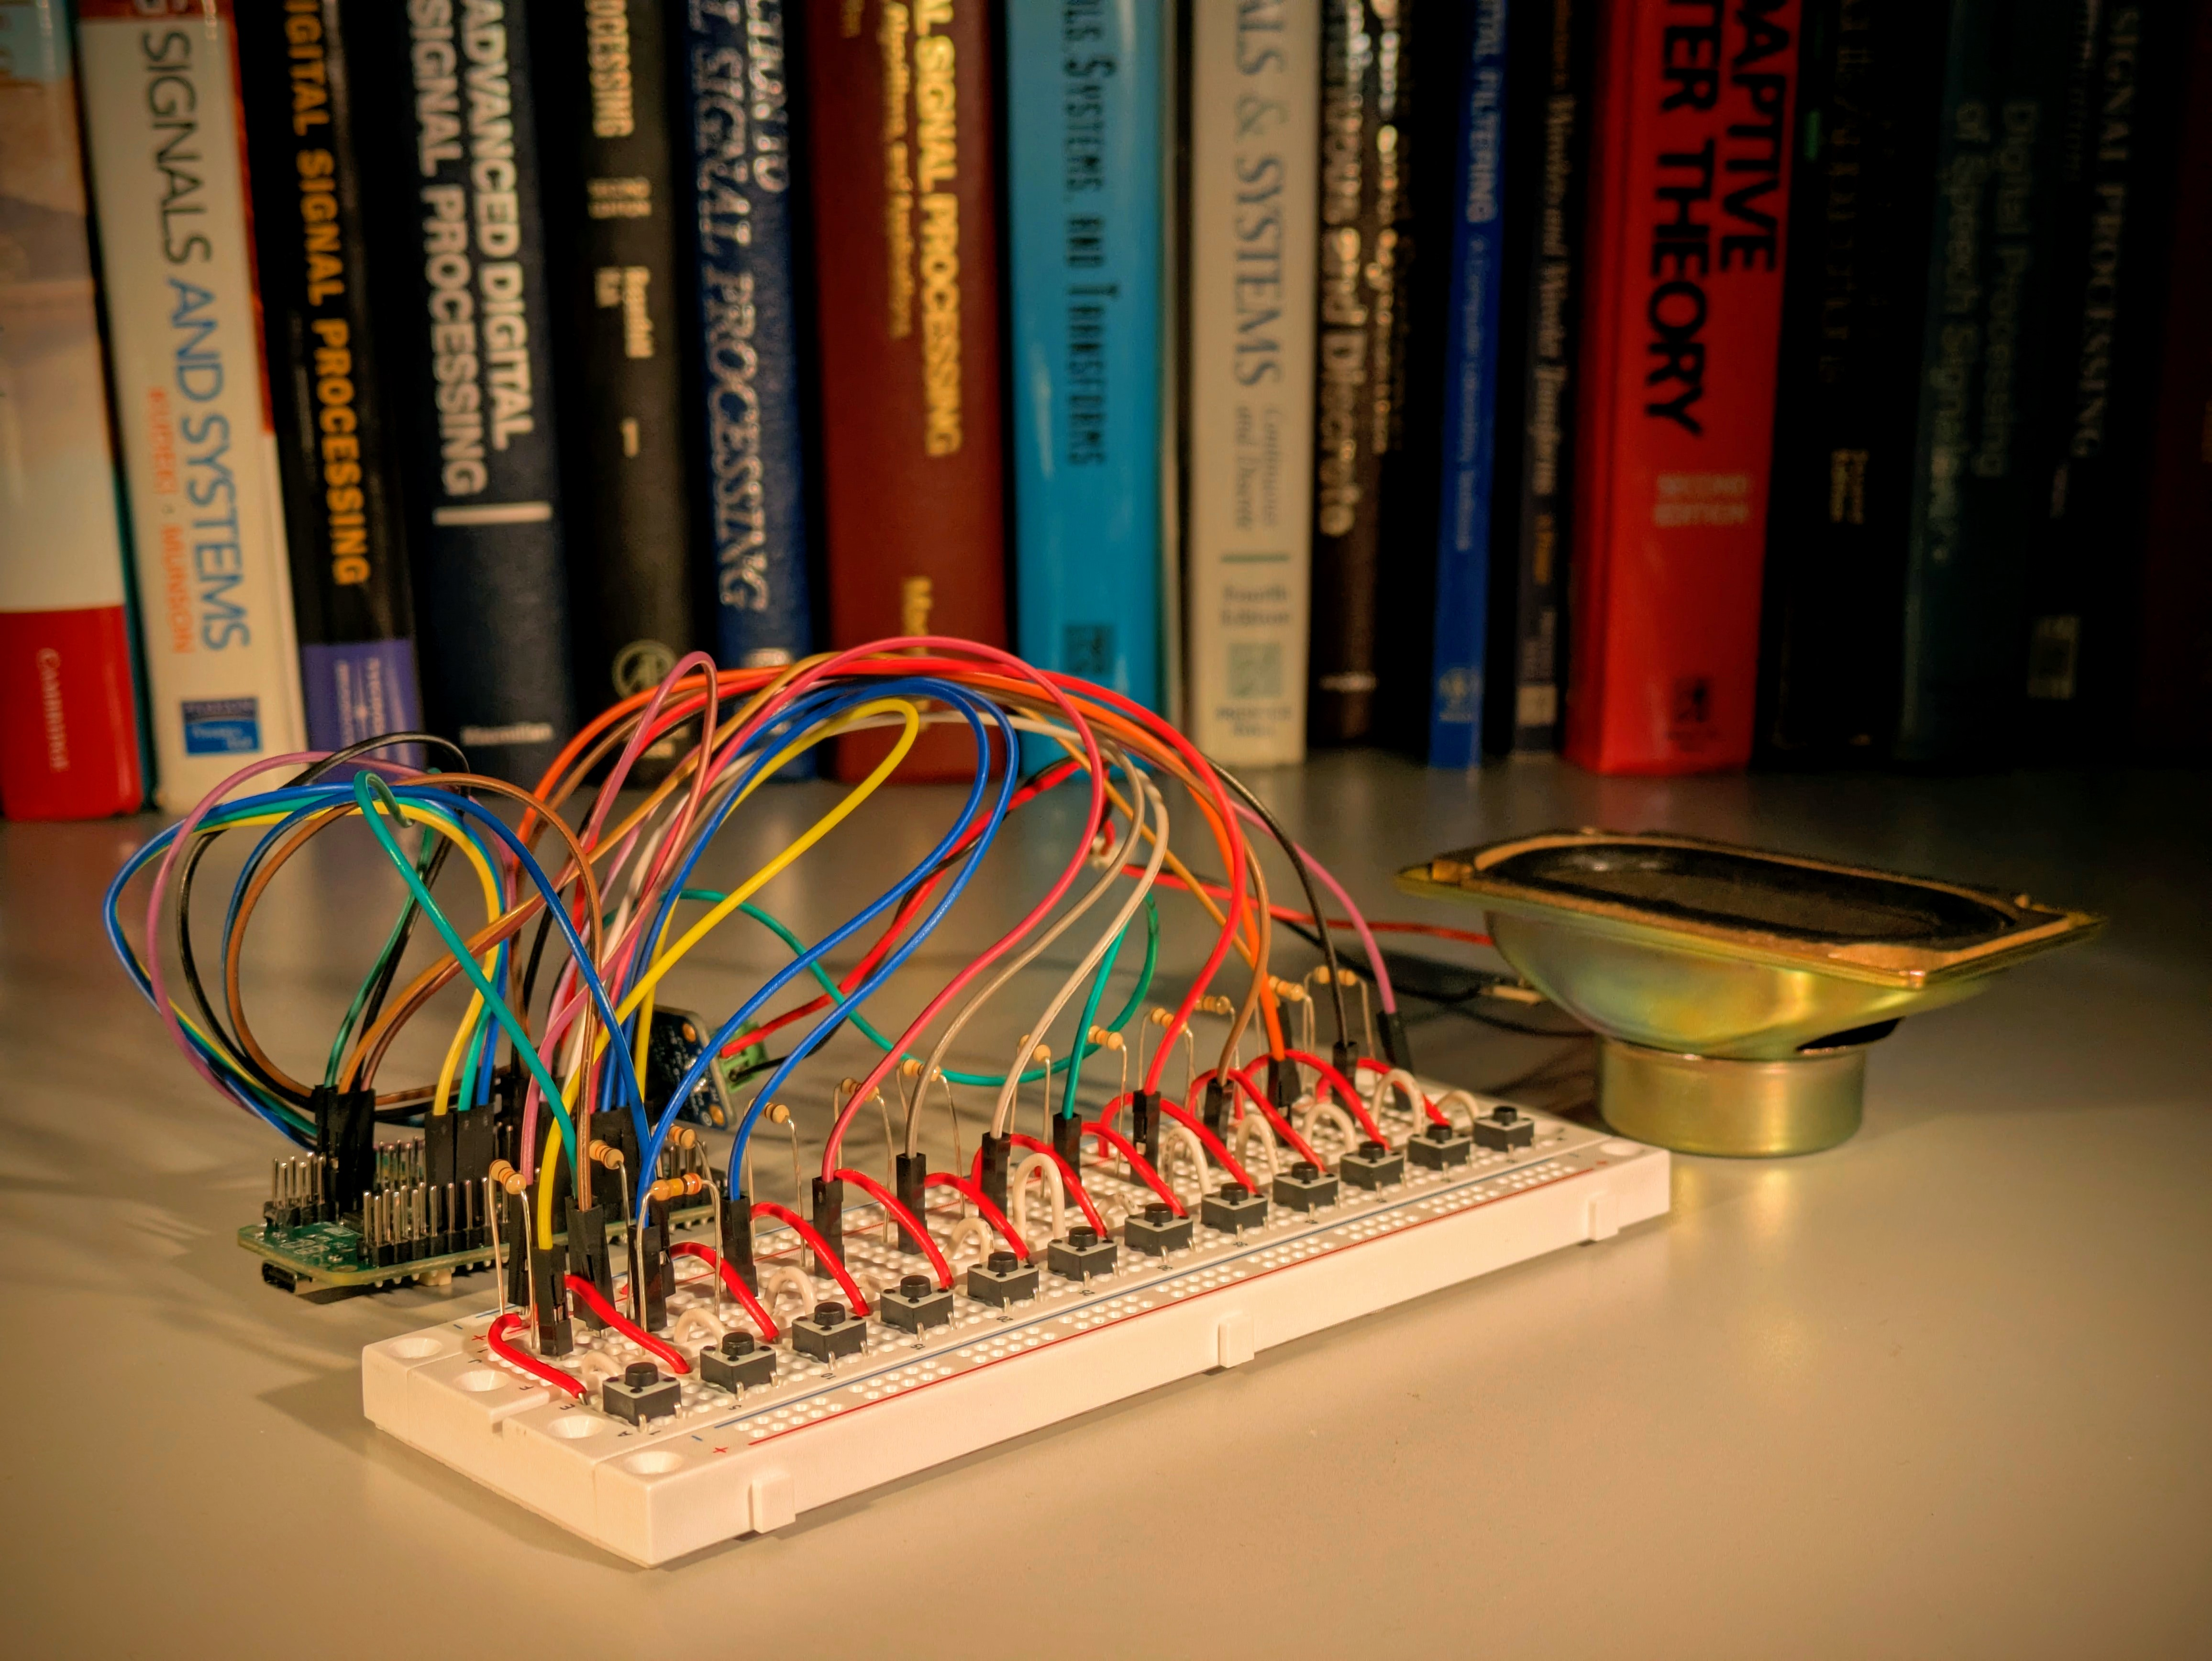
\includegraphics[width=\columnwidth]{breadboard-prototype.jpg}}
\caption{Breadboard Prototype with Pico2-iCE development board}
\label{fig:breadboard-prototype}
\end{figure}

\begin{figure*}[t] 
    \centering
    \includesvg[width=\textwidth]{system-diagram-fixed} 
    \caption{Kympson Model S v2.1 Numerically Controlled Oscillator Diagram}
    \label{fig:nco-diagram}
\end{figure*}

\subsection{Dividing the Main Clock}
The Kympson Model S v2.1 is reliant on a master clock to operate. This master clock runs at 24.576 MHz; however, other processes in the system require different clock rates. The sample generation pipeline requires a 48 kHz clock. The I\textsuperscript{2}S transmission also needs a 1.536 MHz bit clock as the bitstream runs at 32 times the sample rate.

These divisions of the master clock are produced by the clock divider module located in the clock\_divider.sv file of the source code~\cite{github-release}. While it may seem most intuitive to simply use a counter to generate the new, slower clocks, this can produce timing inconsistency with the master clock as any derivative clocks can be slightly delayed.

Instead, as has been done with the Kympson Model S v2.1, clock enable outputs are generated. These clock enable outputs are brought high when every rising edge of a slower, derivative clock should be. This clock enable signal can then be combined with the master clock with a logical AND operation to provide a stable, slower clock signal to any module that requires it without any delayed timings that may cause problems.

\subsection{Obtaining Digital Input from Key Presses}
The Kympson Model S v2.1 has 13 buttons. These buttons are pulled down externally with 11k$\Omega$ resistors, and when pressed bring each logic input to 3.3V.

An important thing to be aware of when using buttons is bouncing. When a button is pressed, the internal contacts often bounce physically before making solid contact. This creates a series of false 'on/off' signals before the circuit stabilizes. If the downstream logic is not designed to tolerate these bounces, it may perceive that the button was pressed many times in succession when it was actually only pressed once. For a deeper exploration into button bouncing and debouncing, look to the fantastic, comprehensive overview by Ganssle in~\cite{ganssle2004guide}.



There are many methods of button debouncing. Most methods solve the issue by delaying signal edges until the button signal is stable, lengthening the on-duration of any rising edges (delaying falling edges), or a combination of both. The Kympson Model S v2.1 utilizes the first of these methods.  

The Kympson Model S v2.1 is designed to tolerate bouncing using the debouncer module, which is located in debouncer.sv in the source code~\cite{github-release}. For each of the 13 keys, a debouncer module is instantiated. This debouncer takes in each button's raw digital value, and any time the button changes state it starts a timer. That timer is set for about 6 milliseconds. When the raw value hasn't changed for that 6 millisecond time threshold, i.e., the timer has incremented past 6 milliseconds, the debouncer module updates that button's debounced logic signal. These debounced button logic signals are then passed along to the tone-frequency-calculator module.

\subsection{Calculating the Accumulator Increment Value}
The accumulator increment value is what decides what the frequency of the output waveform will be. A smaller increment value will cause the phase accumulator to iterate through the NCO waveform LUT slower, resulting in more samples per period, thus giving a longer period and reduced frequency. By extension, a larger increment value will cause the phase accumulator to iterate through the NCO waveform LUT faster, resulting in fewer samples per period, thus giving a shorter period and increased frequency. 

Located in tone\_frequency\_calculator.sv in the source code~\cite{github-release}, the tone frequency calculator module receives debounced button logic signals from the debouncer module, and depending on the key that is pressed, a different accumulator increment value will be sent to the NCO. For a given frequency $f_{desired}$, the formula for the phase increment is given by 
\begin{center}
    $increment = \frac{N\times f_{desired}\ (Hz)}{F_s\ (Hz)}$
\end{center}
where N is the number of samples in the waveform ROM. In the FPGA, this is represented by a 32-bit fixed point number with 5 whole number bits and 27 fractional bits.


\subsection{The Numerically Controlled Oscillator}
The numerically controlled oscillator is contained within the nco.sv file of the source code~\cite{github-release} and runs in cycles. It starts a cycle once at every rising edge of the sample clock (48kHz) provided by the clock divider module. The steps within each cycle are defined by a state machine. The state machine runs at the much faster master clock rate (24.576 MHz). Within the state machine are the phase calculation, LUT reading, multiplication and linear interpolation processes.

%This module receives a reset, master clock, sample clock, mute, and accumulator increment value. Its only output is the sample output which is sent to the I\textsuperscript{2}S transmitter module.


\subsection{Calculating the Phase}
Like a standard numerically controlled oscillator implementation, the accumulator register is incremented by the accumulator increment value every cycle (48 kHz). This accumulator register output is a fixed point value as described before. The whole part of the accumulator is used to address the ROMs, and the fractional part is used for the linear interpolation.

%The phase value of the accumulator is fixed point. That means that a certain number of the most significant bits, in this case 5, are considered the whole number part, and the rest of the lesser significant bits, in this case 27, are considered the fractional part.

\subsection{Reading the ROMs}
The Kympson Model S v2.1 is designed with two 16-bit length-32 ROMs: one stores coarse sample data, and the other stores the slope in-between each coarse sample data point from the first ROM. This allows for linear interpolation to be performed without the need for division and subtraction to calculate the slope every time.

The 5-bit whole part of the accumulator phase value is brought into the address input of both LUTs. The output of the waveform sample LUT is the coarse sample output at the given point in phase.

As for the slope ROM, the concept of storing the slope in a LUT was first tested in Python. In this test, the slope was calculated by taking the derivative of the sinusoidal sample data. This produced promising results, but as can be seen in Fig.~\ref{fig:derivative-graph} the output waveform has a minuscule sawtooth quality. This is caused by the derivative not being the same as the point to point slope. Additionally, an off-by-one error exists in the Python test resulting in the NCO output becoming offset from the LUT data. Instead of using the derivative, the slope between coarse sample points was used. This removed the sawtooth effect.

In an effort to more efficiently utilize ROM space, the slope LUT does not simply hold the point-to-point slope, but rather holds the point-to-point slope multiplied by 4. This is because for a 32-sampled sinusoidal wave, which is currently the only wave programmed into the Kympson Model S v2.1, the largest the change in sample values per 1/32 of a period will be about 6389. This is only about 20\% of the space provided in the slope ROM. In an effort to maximize slope precision, the values in the slope LUT are multiplied by 4 when generated in Python so that more bits are used to represent the slope.

\begin{figure}[H]
\centerline{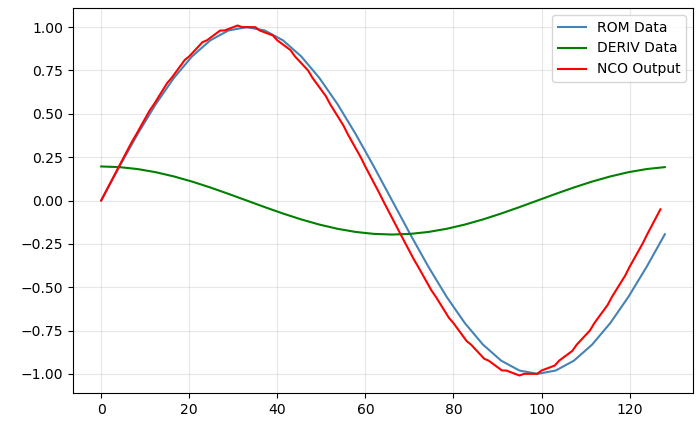
\includegraphics[width=\columnwidth]{derivative-graph.png}}
\caption{Python Graph of NCO Derivative Theory}
\label{fig:derivative-graph}
\end{figure}

\subsection{Linear Interpolation}
The outputs from the two LUTs are used to perform linear interpolation. This follows the equation for a line $y=mx+b$. The slope from the slope LUT ($m$) and the fractional part of the accumulator ($x$) are multiplied together.

It must be kept in mind that the multiplication process of Booth's Radix 4 does not inherently keep track of any decimal places, so after the multiplication is performed, the raw product must be bit shifted right to divide while being sign extended for the most significant bits. This is done a total of 29 times: 27 for the 27-bit fixed point accumulator value, and another 2 because the slope was pre-multiplied by 4. This gives the true product.

After the multiplication is over, the product is added to the coarse sample value from the waveform LUT ($b$). The sum is the final sample output, seen in Fig.~\ref{fig:nco-testbench}.

\begin{figure}[H]
\centerline{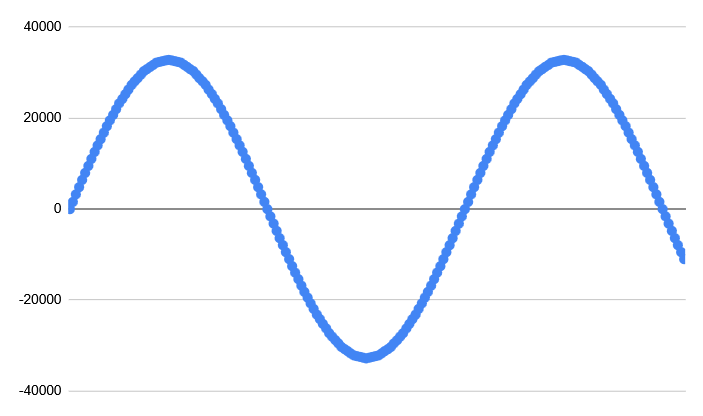
\includegraphics[width=\columnwidth]{nco-testbench.png}}
\caption{NCO Testbench Output Samples}
\label{fig:nco-testbench}
\end{figure}

While the testbench output seen in Fig.~\ref{fig:nco-testbench} does appear to be very sinusoidal, by performing linear interpolation, the result is not a perfect sine wave. Breaking the desired waveform into 32 samples and interpolating between them introduces harmonic distortion. This can be visualized in Fig.~\ref{fig:interpolation-error} where the sample data is displayed on the upper graph, and the difference between the linearly interpolated data and the actual desired sine wave is displayed on the lower graph. The desired sine wave has a peak-to-peak amplitude of 2\textsuperscript{16} or 65536 counts. The error is small with a maximum error of 157.2 counts, and a root-mean squared error of 81.5 counts.



\begin{figure}%[H]
\centerline{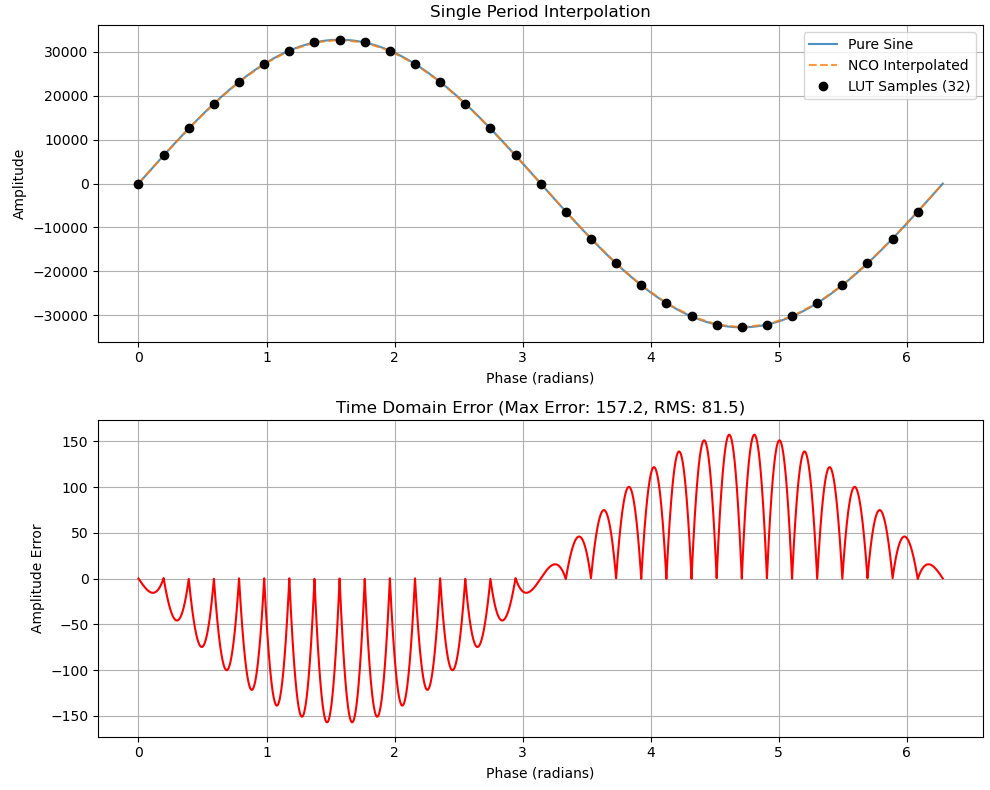
\includegraphics[width=\columnwidth]{interpolation-error.png}}
\caption{Error Introduced by Linearly Interpolating between Samples}
\label{fig:interpolation-error}
\end{figure}

To further look at the error introduced by the linear interpolation, a Fourier transform can be performed to the NCO output data. The result of this can be seen in Fig.~\ref{fig:fourier-transform}. This displays the amplitude of all frequencies in decibels. The fundamental frequency comes in with an expected amplitude of 0 dB, and the harmonic distortion falls just above the -60 dB mark. By more precisely finding the distance in decibels from the fundamental to the highest-amplitude harmonic, the spurious free dynamic range can be calculated to be 59.5 dBc. That means the distance between the loudest harmonic and the carrier (fundamental) is 59.5 dB. This is a very good result.

\begin{figure}%[H]
\centerline{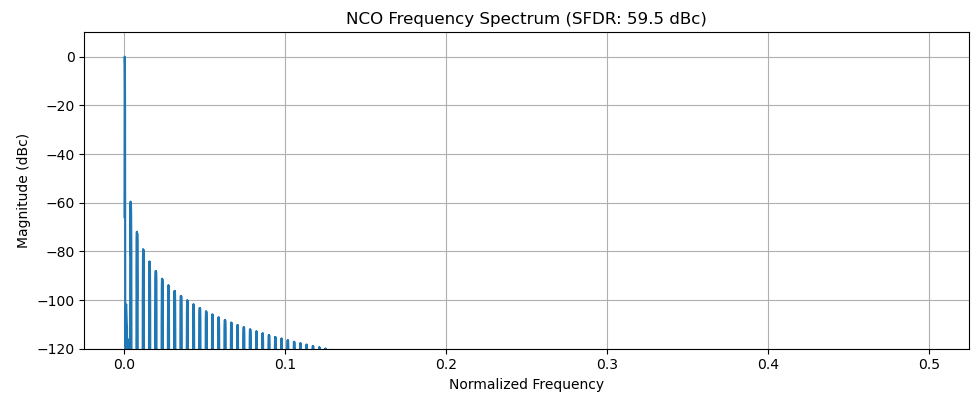
\includegraphics[width=\columnwidth]{fourier-transform.png}}
\caption{Harmonic Distortion Visualized with a Fourier Transform}
\label{fig:fourier-transform}
\end{figure}

\subsection{Multiplication with Modified Booth's Algorithm (Radix 4)}
SystemVerilog has a multiplication operator that can be used with the * character. The Kympson Model S v2.0 was created before v2.1 as a test of the NCO logic using this built-in multiplication operator. However, this multiplication, once synthesized into logic, is purely combinational logic. That means that the multiplication will be physically implemented in the FPGA as purely logic gates and will take less than one clock cycle to execute. While this is ludicrously fast, doing multiplication this way takes up a lot of space on the FPGA, and there are a multitude of clock cycles that could be used for a slower alternative.

Additionally, part of the scope defined for this project was to implement the multiplication manually using Booth's Algorithm. Rather than standard Booth's Algorithm Radix-2, modified Booth's Algorithm, also known as Booth's Algorithm Radix-4 was implemented inside the NCO module as part of the state machine due to being more time-efficient than Radix-2.

The modified Booth's Algorithm implementation requires an even number of input bits, as the number of cycles performed is half of the bit-length of the largest input value. If the raw 27-bit value's length was used, the calculated number of cycles would be a fraction. Because of this, the 27-bit value must be sign extended to 28 bits. This gives 14 total modified Booth's Algorithm Radix-4 cycles.

The state machine also requires another two cycles for Booth's algorithm to initialize registers and another cycle at the end to push the final output to the sample output register and send the state machine to the next step in the NCO process.

\subsection{Outputting the Sample over I\textsuperscript{2}S}
Located in the i2s\_transmitter.sv file in the source code ~\cite{github-release} is the I\textsuperscript{2}S transmitter module. This module receives sound samples from the NCO and outputs them to the DAC via I\textsuperscript{2}S. The I\textsuperscript{2}S protocol consists of three signals: Serial Clock (SCK), Word Select (WS), and Serial Data (SD) ~\cite{nxp_i2s_2022}. SCK is the clock that defines the bit intervals for WS and SD. The SD line is used to send audio sample bits. The bit-depth of the sound samples being sent does not have a defined range by the protocol itself, but I\textsuperscript{2}S devices have defined bit-depth values that they will accept, often being standard values such as 16-bit, 24-bit, etc. WS is used to indicate whether the current sample being sent on SD is for left-channel audio or right-channel audio, with a low (0) indicating left-channel audio and a high (1) indicating right-channel audio. The logic of the I\textsuperscript{2}S protocol requires that WS switches between 0 and 1 (left and right) every x bits, lined up with the end or beginning of each audio sample, where x is the bit-depth of the samples being sent. Additionally, WS is to transition from 1/0 to 0/1 (left- to right- or right- to left-channel) 1 SCK period before the most-significant bit (MSB) of the next sound sample. This is all shown visually in Fig.~\ref{fig:i2s_bit_diagram}.

%This module receives a sound sample input from the NCO, and it also receives a master clock and reset signal. It outputs on 3 data lines defined by the I\textsuperscript{2}S protocol.


\begin{figure}[H]
\centerline{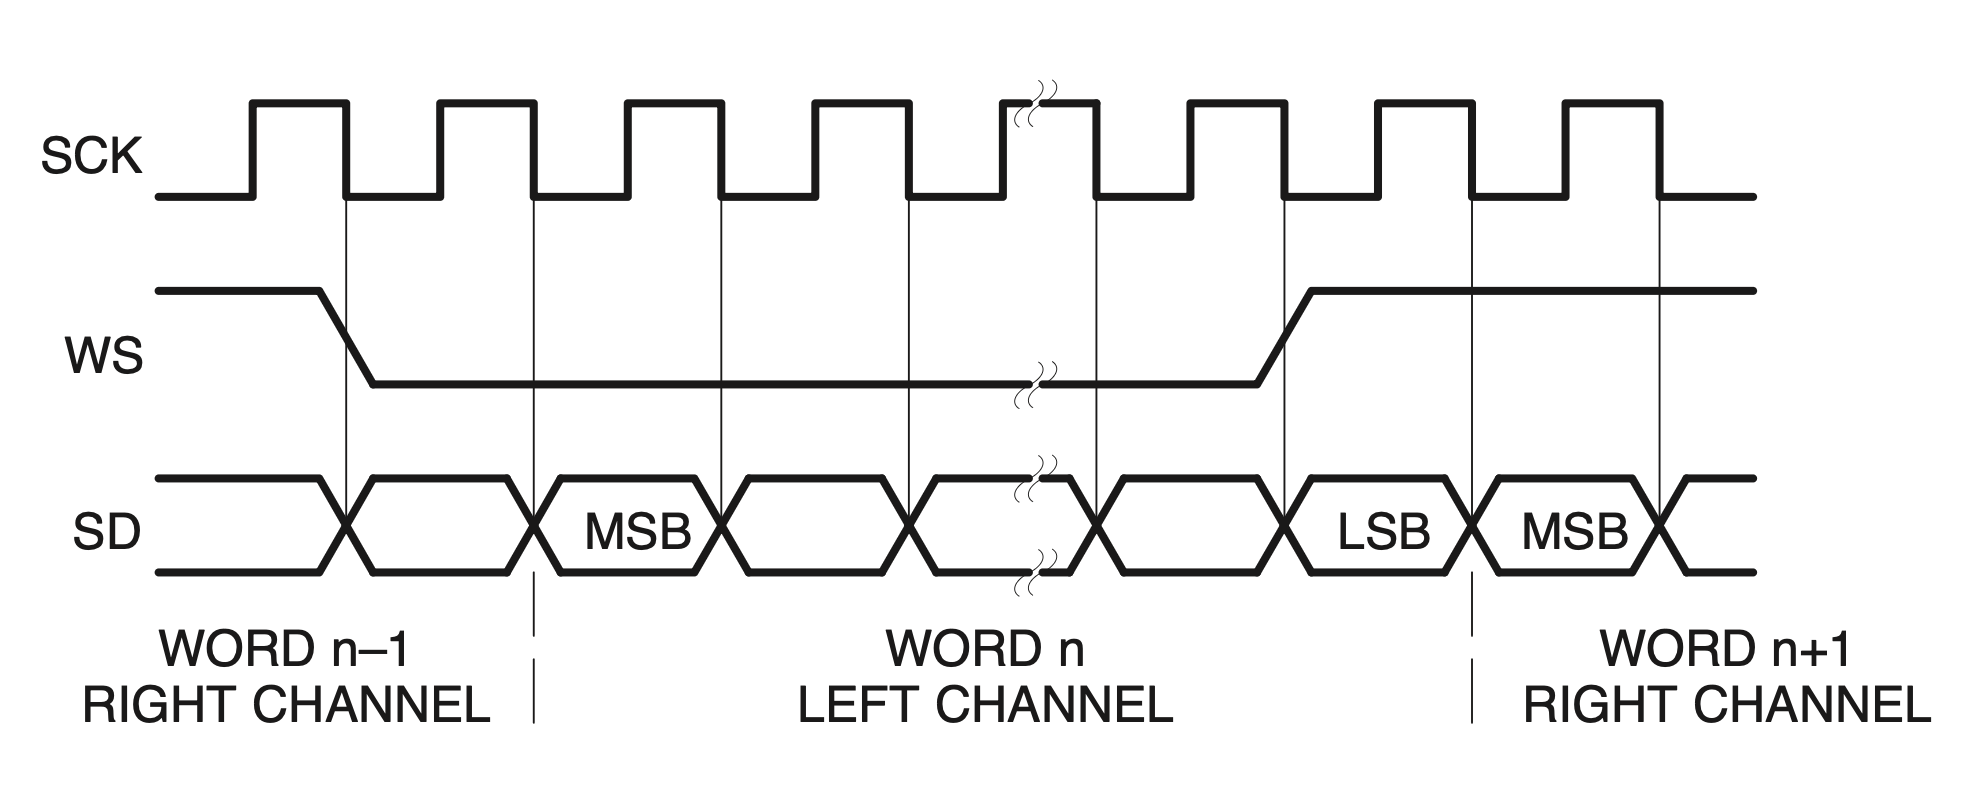
\includegraphics[width=\columnwidth]{I2S-bit-diagram.png}}
\caption{I\textsuperscript{2}S Data Lines \cite{nxp_i2s_2022}}
\label{fig:i2s_bit_diagram}
\end{figure}

The Kympson Model S, using I\textsuperscript{2}S, sends out 16-bit audio samples (for both left- and right-channel) at sample rate $F_s$ = 48 kHz. This gives us:
\begin{center}
    SCK rate = 48 kHz $\times$ 32 bits = 1.536 MHz
\end{center}
In the FPGA, this is done using a state machine and a 5-bit counter to keep track of the 32 total sound sample bits being sent (16 bits per sample, two samples: one for left and one for right). 

The audio sample data is sent via I\textsuperscript{2}S to the MAX98357A IC. As can be seen in the IC's datasheet ~\cite{max98357_datasheet}, the MAX98357A is able to decode the I\textsuperscript{2}S data and with a variable gain, use a class D amplifier structure to output it to a speaker. Class D amplifiers, also known as switching amplifiers, use pulse-width modulation (PWM) or similar techniques to efficiently produce analog signals with digital circuitry. The PWM output of the MAX98357A relies on the inductance of the speaker as a low-pass filter to produce the desired analog current and thus analog speaker cone vibrations. In order to measure the output and display it on an oscilloscope, the current through the speaker has to be measured rather than the voltage. If voltage were measured, the oscilloscope view would look nothing like the desired waveform. It would show the unfiltered PWM output of the DAC. Viewing the current, however, proves the faithfulness of the output of the Kympson Model S v2.1 to the desired waveform as can be seen in Fig.~\ref{fig:analog-scope}.

\begin{figure}[H]
\centerline{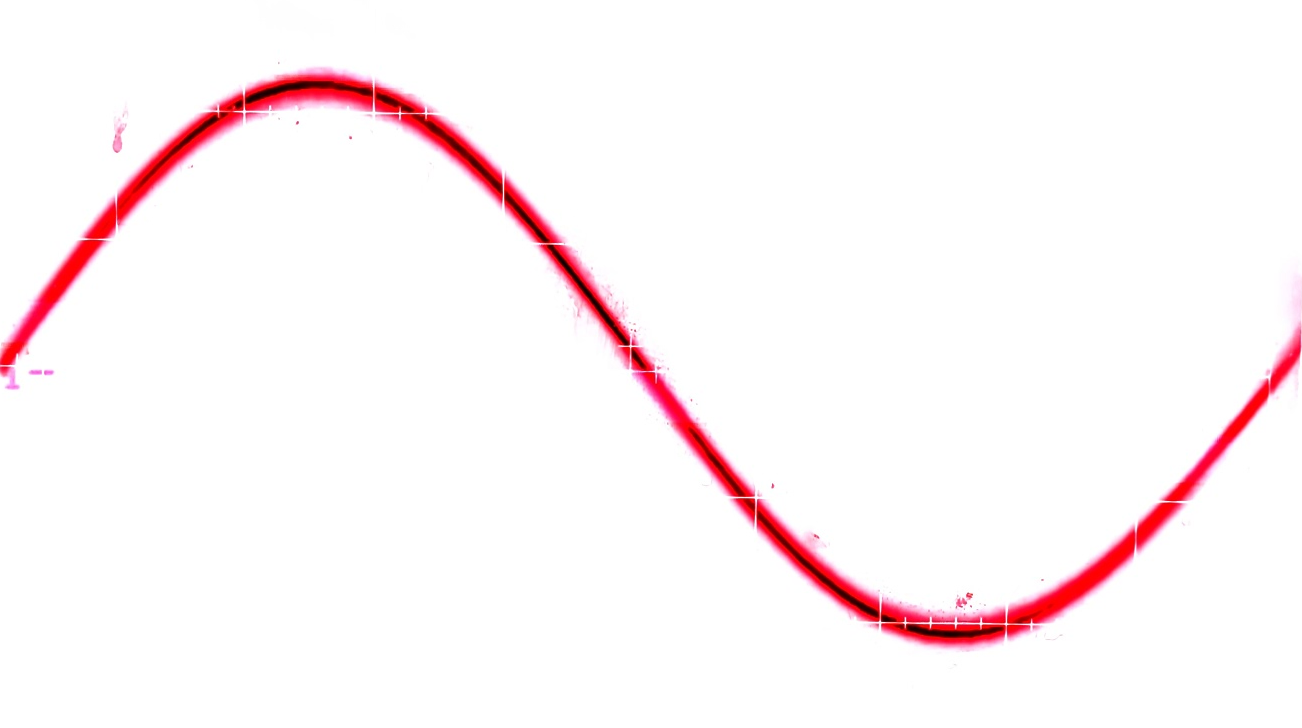
\includegraphics[width=\columnwidth]{analog-scope-inverted.png}}
\caption{Analog Oscilloscope View of Current Through the Output Speaker}
\label{fig:analog-scope}
\end{figure}

\section*{Conclusion} % I think the * here makes there be no roman numeral
The Kympson Model S v2.1 does exactly what it was made to do: it reliably generates an accurate wave in both frequency and shape. It is also incredibly flexible because the NCO allows it to produce any periodic waveform. Because the framework for wave generation and audio transmission are now established, the Kympson Model S provides a reliable and flexible foundation upon which further development can be done, whether that be for alternate methods of reading key input, digital signal processing on the sound being generated, or anything else.


% Peter's ideas for improving things in the future:
% Add shift registers for keys --> unlimitted keys (and modular too maybe?)
% Add more built in waveforms and ability to cycle through
% Maybe ability to interpolate between different waveforms (this would be so cool, could be another fader/knob)
% Pitch bend and modulation (like a leslie cabinet on an organ) knobs
% ADSR envelope
% Volume knob
% Stereo audio production (different left and right channel things: freq, waveform, volume, adsr)
% line level, headphone, and speaker level outputs

\bibliographystyle{IEEEtran}
\bibliography{references}

%\begin{thebibliography}{00}
%\bibitem{b1} Philips Semiconductors, I2S bus specification, Jun. 1996.
%\end{thebibliography}

\end{document}
